
\subsection{The Segway System}
The segway was constructed using a metal plate as foundation for the robot.
The motors were then attached to the lower side of the plate.
On top of the basis was then mounted the PCB designed with the two H-bridges to control the two motors.

A second layer was then added as a plug-in module to which the different components could be plugged in and the power supply converting the input voltage to a 5V supply for the FPGA.
This layer included a plug for the FPGA and the IMU.
Furthermore was there added plugs for a bluetooth sender/transmitter and two wheel encoders, but due to time constraints was their functionality not required at the given time and hence not added to the final system.

A sketch of the final segway is seen in figure \ref{fig:segwaysketch}.

\begin{figure}[H]
\centering
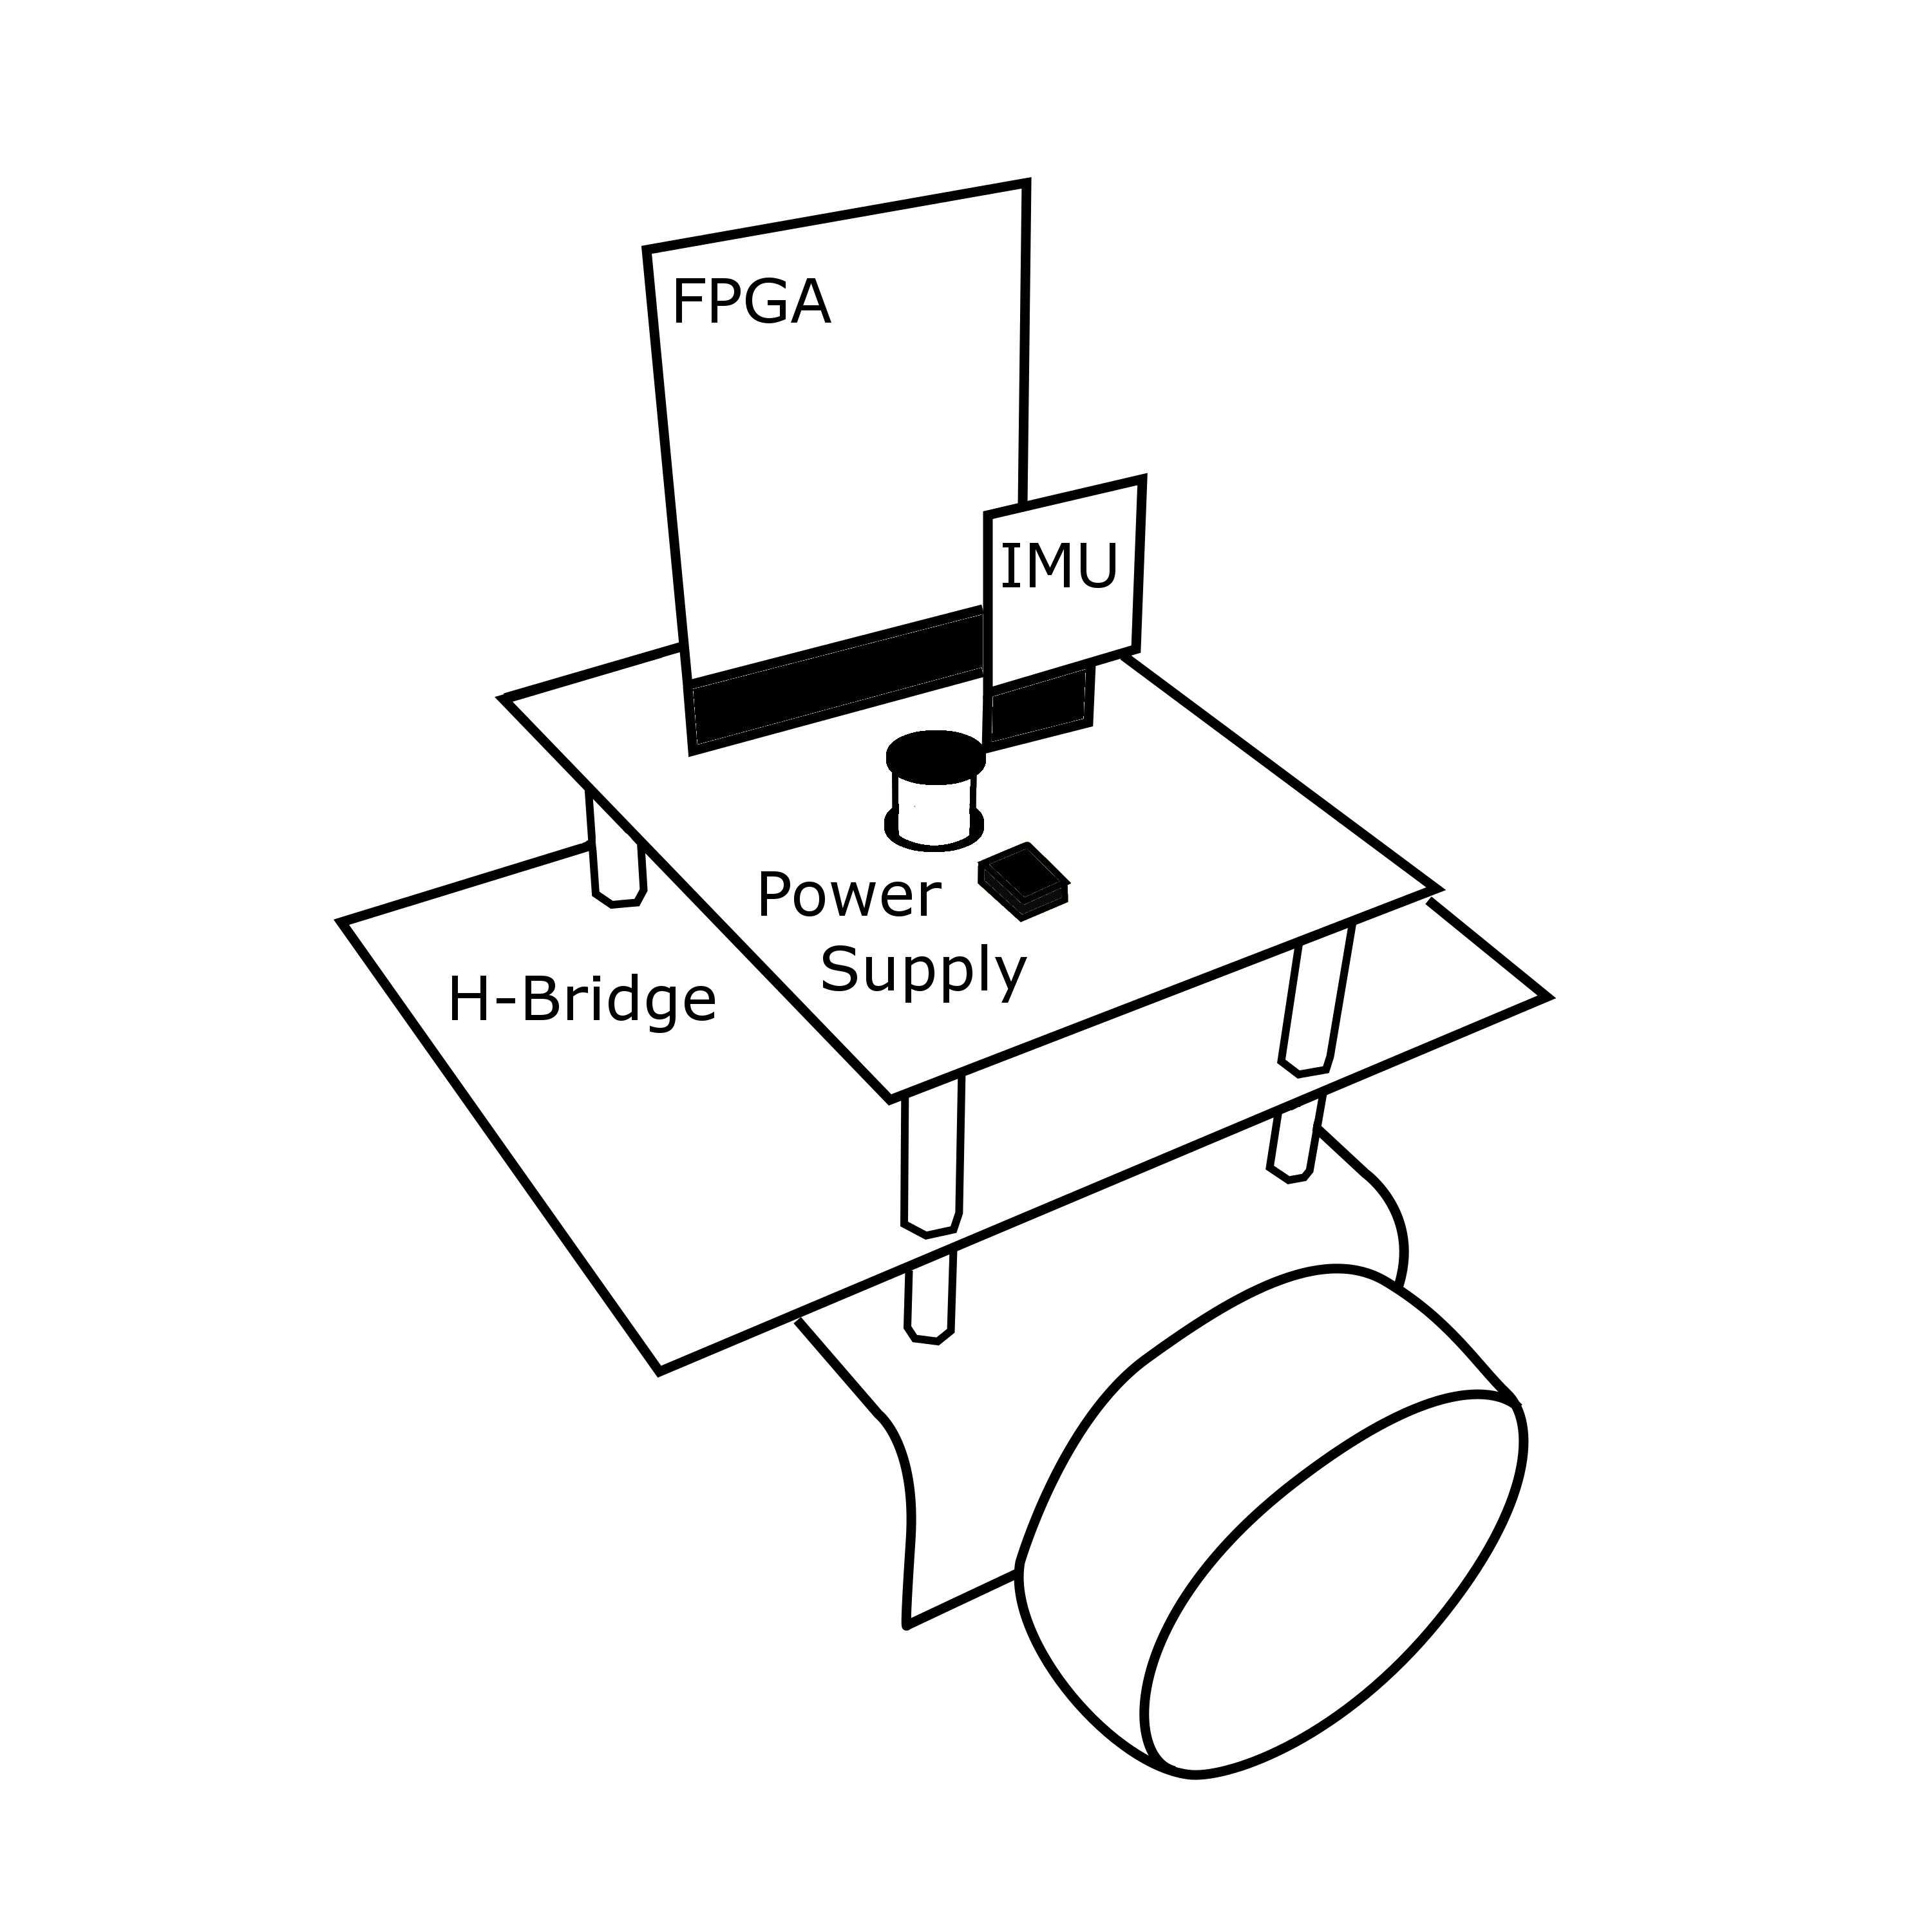
\includegraphics[width = 0.5 \textwidth]{images/segway}
\caption{Sketch of the build segway.}
\label{fig:segwaysketch}
\end{figure}